\chapter{Entorno empresarial} \label{empresa}
En este capítulo se presenta una descripción del entorno en el cual se desarrolló el proyecto de pasantía en la empresa iKêls Consulting. Comprende una breve reseña histórica, su misión y visión, la estructura organizacional y el área a la cual el pasante estuvo asignado.

\section{Antecedentes de la empresa}
IKêls Consulting \cite{ikels} se creó el año 2008 como una empresa dedicada al desarrollo de soluciones en el área de Sistemas de Información. Los fundadores contaban con una amplia trayectoria en los procesos y tecnología para la elaboración de documentación técnica avanzada que brindaron las bases para entender los retos de la administración de contenidos complejos, dinámicos y voluminosos (por ejemplo las normas técnicas de ingeniería de PDVSA que abarcan más de 20.000 páginas de textos, planos, tablas, imágenes, etc. perfectamente indexadas).
Fueron pioneros en desarrollar páginas web dinámicas en el país para empresas como British Petroleum (BP) y contaban con su propio CMS \cite{cmsBarker}) llamado WALK. Sin embargo en el camino se encontraron con Umbraco \cite{umbraco}, cuya plataforma resultó calzar perfectamente con las habilidades y expectativas de la empresa. 

Para aprovechar la experiencia previa los productos y servicios que ofrece iKêls Consulting \cite{ikels} se concentran en el área de aplicaciones web (por ejemplo, sistemas de manejo de contenido o CMS \cite{cmsBarker}) para el sector corporativo atendiendo a un selecto grupo de clientes con presencia local e internacional.
Actualmente, las actividades principales se concentran en:

\begin{itemize}
 \item Construcción de portales web en múltiples idiomas y que pueden ser administrados por sus propios dueños. Esto incluye la programación de módulos especiales para integrar información desde y hacia sistemas externos, desplegar datos de manera amigable o generar notificaciones automáticas dependientes de actividades de los visitantes u otros eventos.
 \item Apoyo en la gestión de contenido de portales web.
 \item Consultoría y gestión para optimizar las variables asociadas al rendimiento y desempeño de las páginas web, teniendo especial interés en el monitoreo de presencia en buscadores, evaluación del perfil de los visitantes y garantizar un nivel adecuado de usabilidad en diferentes dispositivos, etc.
 \item Desarrollo de productos personalizados que complementen las ventajas y facilidades de los dispositivos móviles en sincronización con mecanismos de soporte en servidores web.
 \item Desarrollo de soluciones especializadas para ofrecer bajo el modelo SaaS o \textit{Software as a Service} (Software como servicio) \cite{saas}.
\end{itemize}

\section{Misión}
Proveer productos y servicios en el área de sistemas de información que permitan una comunicación efectiva de nuestros clientes con su público y también sirva como plataforma de trabajo donde se aprovechen las innovaciones y ventajas de las tecnologías más modernas \cite{ikels}.

\section{Visión}
La empresa busca ser un proveedor confiable, que ofrece un alto valor agregado en cada producto o servicio que prestamos a nuestros clientes \cite{ikels}.

\section{Ubicación del pasante}
El proyecto de pasantía pertenece al grupo de Desarrollo de Aplicaciones y cuenta con la dirección del Presidente de la Empresa y con el apoyo de los ingenieros líderes del grupo. A continuación se muestra el organigrama de la empresa.


\pagebreak
\section{Organigrama}
\begin{figure}[hbt]
\begin{center}
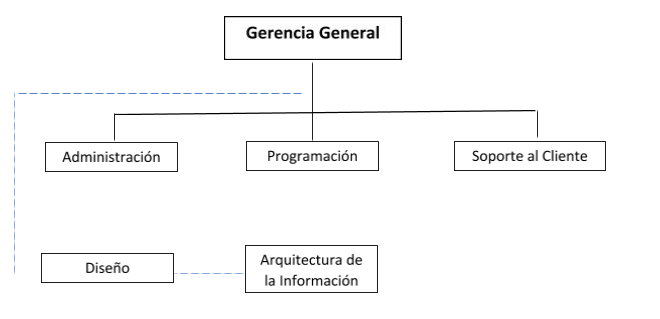
\includegraphics[scale=0.8]{organigrama}
\caption{Organigrama de la Empresa. Fuente: Elaboración propia.}
\label{fig:figura1}
\end{center}
\end{figure}
